% глава = section, параграф = subsection
\documentclass[a4paper,article,14pt]{extarticle}

% главный пакет с шаблоном
\usepackage{spbudiploma}

% Пакеты по желанию (самые распространенные)
\usepackage{cmap} % поиск по документу
\usepackage{amsmath} % уравнения
\usepackage[pdftex]{graphicx} % картинки

\usepackage{textcomp}

\DeclareMathOperator{\logit}{logit}

\begin{document}


\newgeometry{left=30mm, top=20mm, right=15mm, bottom=20mm, nohead, nofoot}
\begin{titlepage}
\begin{small}
\begin{center}

{Санкт-Петербургский государственный университет}

\vspace{30mm}

\textbf{\textit{БАДМАЕВ Артем Тимурович}} \\[8mm]
% Название
\textbf{Выпускная квалификационная работа}\\[3mm]
\textbf{\textit{Построение вероятностной модели возникновения лесных пожаров на основе природных факторов и антропогенной нагрузки}}

\vspace{20mm}
Уровень образования: \textit{бакалавриат}\\
Направление \textit{50.03.01 «Искусства и гуманитарные науки»}\\
Основная образовательная программа \textit{СВ.5045.2019 «Свободные искусства и науки»}\\
Профиль \textit{«Компьютерные науки и искусственный интеллект»}\\[25mm]


% Научный руководитель, рецензент
\begin{flushright}
\begin{minipage}[t]{0.55\textwidth}
{Научный руководитель:} \\
доцент, кафедра проблем конвергенции \\естественных и гуманитарных наук, \\к.ф.-м.н., Князева Ирина Сергеевна

\vspace{10mm}

{Рецензент:} \\
ФГБУН Главная (Пулковская)\\ астрономическая обсерватория РАН, \\к.ф.-м.н., Волобуев Дмитрий Михайлович
\end{minipage}
\end{flushright}

\vfill 

{Санкт-Петербург}
\\{2023}
\end{center}
\end{small}
\end{titlepage}
\restoregeometry
\addtocounter{page}{1}



\tableofcontents


\pagebreak
\specialsection{Введение}

Данная работа посвящена прогнозированию возникновения лесных пожаров. Из года в год масштабные лесные пожары в России привлекают внимание множества людей и сопровождаются волной публикаций в прессе. Это особенно заметно в последние годы на фоне крупнейших в истории пожаров. По данным системы спутникового мониторинга ИСДМ-Рослесхоз в 2019 году пройденная огнем площадь приблизилась к рекорду 2012 года, превысив 15 млн га \cite{2019GodMozhet2019}, а в 2021 был поставлен абсолютный рекорд за историю спутниковых наблюдений — площадь, пройденная огнем, превысила 18 млн га \cite{2021GodPolnyy2021}. Притом последствия явлений таких масштабов не ограничиваются громкими заголовками в прессе и внушительными цифрами статистики. Оба раза густонаселенные районы Сибири накрыло дымом от пожаров на обширных территориях Красноярского края \cite{DymNadSibiryu2019} и Якутии \cite{DymOtLesnyh2021}. Прямой материальный ущерб насчитывал несколько миллиардов рублей \cite{PozharyRossii20212022, YakutiiUshcherbOt2021}. Притом это лишь фактически бухгалтерские оценки ущерба зарегистрированному имуществу, не включающие косвенные убытки, вред здоровью и долгосрочные последствия от рекордного сокращения лесного покрова \cite{MinprirodyOceniliEkonomicheskiy2021}.

Хотя в заявлениях официальных лиц периодически звучат тезисы о том, что лесные пожары являются нормальным природным явлением, а бороться с огнем в труднодоступных районах бессмысленно \cite{KrasnoyarskiyGubernatorNazval2019}, исследования свидетельствуют об обратном. Крупные пожары приводят к выбросу в атмосферу больших объемов дыма и твердых частиц, которые могут значительно влиять на качество воздуха на населенных территориях, притом даже находящихся в сотнях и тысячах километрах от огня, представляя угрозу здоровью населения \cite{EfimovaAssessmentSmokePollution2021}. Кроме того, горение на большой площади и последующее уменьшение лесного покрова вносят дополнительный вклад в изменение климата. Дым и парниковые газы усиливают парниковый эффект, а уничтожение леса ухудшает способность планеты поглощать углекислый газ \cite{XuWildfiresGlobalClimate2020}.

Несмотря на то, что лесные пожары действительно являются нормальной частью функционирования экосистемы тайги, последние десятилетия в результате антропогенных причин и изменения климата частота и масштабы пожаров растут \cite{KharukWildfiresSiberianTaiga2021}. Увеличивается пожароопасный сезон, а погода становится более засушливой, из-за чего снижается влажность топлива. Возгорания происходят чаще, а горение проходит интенсивнее. Масштаб пожаров значительно влияет на биоразнообразие и устойчивость экосистемы. И хотя влияние этих изменений не всегда однозначно негативное, предсказать дальнейший вектор развития при разбалансировке системы проблематично \cite{KharukWildfiresSiberianTaiga2021}.

Расширение промышленного освоения северных районов Сибири также сказывается на состоянии экосистем и пожароопасности региона и ведет к их большей уязвимости \cite{ShvidenkoClimateChangeWildfires2013}. Лесное хозяйство в нынешнем виде является дополнительной угрозой для лесов, так как одной из главных причин возгораний в тайге являются случайные и преднамеренные поджоги на лесозаготовках в силу слабого контроля за соблюдением правил пожарной безопасности \cite{GrinpisPoluchilPervye2021}. Соответственно, изменения в антропогенных факторах дополнительно увеличивают риски лесных пожаров и требуют еще больших ресурсов для наблюдения и контроля за пожарной обстановкой \cite{ShvidenkoClimateChangeWildfires2013}. В добавок, неутешительная динамика пожаров в России обещает еще и рост экономического ущерба для лесного фонда и лесного хозяйства.

Однако рост пожароопасности не единственная причина катастрофических масштабов лесных пожаров последнее десятилетие. Помимо факторов, влияющих на возникновение пожаров, важно учитывать пожароохранный режим и противодействие распространению огня, так как грамотные противопожарные меры позволяют смягчить последствия, минимизировать экономический ущерб и затронутую пожаром площадь. Однако немаловажным фактором успеха является своевременность реагирования. С вышедшим из под контроля пожаром крайне сложно бороться, ибо при масштабах лесов России для этого физически недостаточно ресурсов. Если пожар не удалось сдержать, то фокус обычно смещается на защиту населения, хозяйственных активов, инфраструктуры \cite{AlekseyYaroshenkoVazhno2019}. Поэтому важно своевременно выявлять и реагировать на возникающие очаги, пока они не успели выйти из под контроля.

Однако даже тушение таких небольших возгораний требует значительных усилий из-за обширной суммарной площади лесов и труднодоступности большинства из них, особенно в условиях нынешнего финансирования лесной охраны \cite{GreenpeacePravitelstvuNuzhno2021}. Сильная ограниченность в ресурсах не позволяет удачно справляться с возросшим масштабом угроз. Это вынуждает выделять более приоритетные и менее приоритетные пожары. В России это разделение фактически фиксированное и отражено в делении на четыре зоны мониторинга, которые различаются способами слежения (наземный, авиационный, космический) и предписанными мерами реагирования на обнаруженный пожар \cite{InformacionnayaSistemaDistancionnogo2008}.

Наибольшую критику вызывает так называемая «зона контроля», или зона космического мониторинга 2-го уровня, где осуществляется исключительно спутниковый мониторинг, а тушение пожаров не обязательно. Создание подобных зон оправданная мера, так как действительно, какие-то пожары целесообразно не тушить, тем самым высвобождая ресурсы для других \cite{KtoKontroliruetPozhary2019}. Однако дефицит финансирования вынуждает делать зону контроля неоправданно большой. Именно там при неудачном сочетании погоды и отсутствия реагирования создаются условия для катастрофических пожаров масштаба 2019 и 2021 годов. Крупные пожары регулярно приводят к призывам о пересмотре зон контроля в связи с меняющимися природными и антропогенными условиями, что делает очаги даже в отдаленных районах более опасными \cite{ZonKontrolyaStanet2022}.

Однако такие изменения требуют подробной оценки целесообразности тушения лесных пожаров на той или иной территории. Смысл разделения на зоны — распределить ресурсы пожарной охраны, отдавая приоритет самым опасным пожарам, но притом тем, с которыми реально справиться. Тогда деление должно производиться с учетом потенциальных угроз, имеющихся ресурсов. Так как эти факторы очень изменчивы, будучи зависимыми от погоды, финансирования, поведения людей, то и прогнозирование должно быть достаточно гибким и отражать происходящие сдвиги. На основе подобных прогнозов уже будет осуществляться размещение противопожарных сил, которое позволит минимизировать время реагирования на обнаруженные очаги.

Создание такого прогноза — задача из области моделирования рисков. В качестве составляющих частей такого подхода выделяют моделирование угроз,  подверженность риску, уязвимость и способность к противодействию \cite{OliveiraWildfireRiskModeling2021}. В данном случае угрозы — это, собственно, лесной пожар. Подверженность риску — ценность ценность имущества и активов, которым может быть нанесен ущерб, а уязвимость — собственно потенциальный ущерб при столкновении с угрозой. Способность к противодействию — потенциал для уменьшения угрозы и связанного с ней ущерба.

Притом моделирование лесных пожаров — то есть угроз — можно разделить на два класса: модели возникновения и симуляции распространения. Первые обычно изучаются статистическим аппаратом и являются вероятностными моделями, то есть оценивающими вероятность возникновения пожара или достижения им тех или иных параметров. Тогда как с помощью симуляций строят подробные сценарии дальнейшего распространения огня на макроуровне. Классическим примеров симуляции является Canadian Forest Fire Behavior Prediction System (CFFBPS) \cite{CanadianForestFire}, российским аналогом которой является Информационная система дистанционного мониторинга (ИСДМ-Рослесхоз) \cite{RossiyskayaSistemaSputnikovogo2004}. Другими словами, модели возникновения оценивают вероятность возникновения нового пожара, тогда как симуляции распространения моделируют ожидаемое поведение уже существующего.

Вероятностные модели позволяют оценить вклад различных факторов в пожароопасность региона и инкорпорировать в предсказания неопределенность, неизбежно сопровождающую прогнозирование погоды и природных процессов. Так можно оценивать последствия изменения погоды и климата, влияние режима землепользования на вероятность возникновения пожара, оценивать эффективность мер противопожарной безопасности. Одну из таких вероятностных моделей пожарной активности предложили французские исследователи в рамках созданного ими байесовского фреймворка Firelihood \cite{PimontPredictionRegionalWildfire2021}.

Подход исследователей рассматривает возникновение пожаров как пространственно—временной пуассоновский процесс, где количество пожаров в день в одной ячейке пространственной сетки является целевой переменной и определяляется распределением Пуассона. Параметры распределения в каждой пространственно-временной точке определялись обобщенной аддитивной моделью (Generalized Additive Model, GAM), что позволило учесть нелинейную зависимость параметров распределения от объясняющих переменных.

Притом альтернативным инструментом машинного обучения, который может учитывать нелинейные зависимости целевой переменной от объясняющих, являются нейронные сети, которые также успешно применялись для моделирования пожарной активности. В частности, многослойный перцептрон был использован для аналогичной задачи моделирования вероятности возникновения лесных пожаров в Италии \cite{EliaEstimatingProbabilityWildfire2020}. Рекуррентные нейросети применялись для моделирования динамики развития лесных пожаров в Канаде \cite{LiangNeuralNetworkModel2019}.

Однако задачу предсказания пожарной активности в регионе также можно рассматривать как задачу компьютерного зрения, если интерпретировать пространственную сетку с данными как многоканальное изображение. В таком случае, задачей модели будет сегментация этого изображения — определение границ «объектов», в нашем случае территорий с повышенном риском возникновения пожаров.

Задачу сегментации успешно решает архитектура сверточной нейросети U-Net \cite{RonnebergerUNetConvolutionalNetworks2015}, которая уже использовалась в сфере лесной охраны для сегментации контуров активных лесных пожаров на основе данных дистанционного зондирования Земли \cite{deAlmeidaPereiraActiveFireDetection2021}. Кроме того, данная архитектура может быть использована в задачах попиксельной регрессии, то есть нахождении значений пикселей целевого изображения на основе значений соответствующих пикселей входных изображений \cite{YaoPixelwiseRegressionUsing2018}.

Данная работа ставит своей целью реализовать модель предсказания пожарной активности на лесных территориях Сибири и Дальнего востока на основе архитектуры U-Net, а также сопоставить ее с обобщенной линейной моделью, чтобы оценить компромисс между интерпретируемостью и эффективностью моделирования.

\pagebreak
\section{Моделирование риска лесных пожаров}
\subsection{Проблемы мониторинга и борьбы с лесными пожарами}
  
Географические условия и особенности экономического развития России ставят перед системой лесной охраны значительные вызовы. С одной стороны, большая площадь лесного покрова сама по себе создает условия для возникновения одновременно большого числа пожаров, их длительного горения и распространения. С другой, невысокая плотность населения и инфраструктуры ограничивают возможности по мониторингу и борьбе с лесными пожарами на обширных территориях тайги Сибири и Дальнего Востока, на которые приходится более 90\% пройденной огнем площади \cite{PonomarevChapter10System2015}.

Сочетание этих факторов привело к формированию системы лесной охраны в ее нынешнем виде. Отсутствие дорожной сети в отдаленных районах тайги делает невозможным наземное наблюдение и создание сети аэродромов для воздушного наблюдения, поэтому на значительной площади лесов осуществляется исключительно космический мониторинг \cite{PonomarevChapter10System2015}. Приоритет в тушении отдается пожарам, напрямую угрожающим населенным пунктам и объектам хозяйства, так как ресурсов Авиалесоохраны недостаточно для тушения всех обнаруженных пожаров \cite{KosmicheskiyMonitoringLesnyh2019}. 

Это, в свою очередь, делает возможным возникновение пожаров катастрофических масштабов на обширных территориях тайги. Так как региональные власти имеют право не тушить пожар в случае, если расходы на борьбу с ним превышают потенциальный ущерб, множество очагов в малонаселенных и отдаленных районах Сибири и Дальнего Востока остаются без внимания \cite{KtoKontroliruetPozhary2019}. Несмотря на рекомендации Авиалесоохраны об определении границ «зон контроля» — территорий, на которых можно не осуществлять тущение — субъекты федерации определяют их по своему усмотрению, как правило расширяя за пределы рекомендуемых границ \cite{KosmicheskiyMonitoringLesnyh2019}.

Власти регионов, на которых лежит ответственность за борьбу с пожарами на своей территории \cite{KosmicheskiyMonitoringLesnyh2019}, руководствуются в первую очередь финансовыми и экономическими соображениями, вынуждены прибегать к такой практике в первую очередь по причине недостаточного финансирования \cite{GreenpeacePravitelstvuNuzhno2021}. Ограниченные ресурсы пожарной охраны, в частности авиацию и квалифицированный персонала, требуется держать наготове для борьбы с угрожающими населению пожарами, тем самым жертвуя малодоступными северными лесами \cite{ZonKontrolyaStanet2022}. 

Однако, если на этапе возникновения пожара в отдаленной северной тайге он действительно не представляет немедленной опасности, то в отсутствие всякого противодействия рискует достичь масштабов, которые будут представлять даже большую угрозу населенным пунктам и экономическим активам. Экономический анализ потенциального ущерба свидетельствует как раз о том, что вышедшие из-под контроля крупные пожары могут представлять больший риск, который, однако трудно оценить на этапе их возникновения \cite{MnimoyRealnoyEkonomicheskoy2019}.

Кроме того, несмотря на частую критику зон контроля, эксперты не отрицают необходимость ее существования как таковой \cite{MnimoyRealnoyEkonomicheskoy2019, GreenpeacePodgotovilPredlozheniya}. Возражения вызывают в первую очередь нынешние границы и площадь этих зон, тогда как само их наличие (только в ином виде) видится необходимым из-за уже упомянутой невозможности обеспечить авиационный мониторинг и своеврменное реагирование на всей территории тайги \cite{PonomarevChapter10System2015, MnimoyRealnoyEkonomicheskoy2019}. Так, Авиалесоохрана с 2015 года рекомендует определять зоны контроля по границе зоны космического мониторинга второго уровня — территорий, где регулярное патрулирование и обязательное тушение пожаров не предусмотрено изначально, и возможно лишь по решению органов власти субъекта \cite{MetodicheskieRekomendaciiPo2010}. Однако на деле власти регионов определяют зоны контроля в том числе на территориях зон космического мониторинга первого уровня \cite{KosmicheskiyMonitoringLesnyh2019}, где Авиалесоохраной ранее предусматривалась борьба с пожарами средствами авиации \cite{MetodicheskieRekomendaciiPo2010}.

Все вышеописанное означает, что задача космического мониторинга труднодоступных лесов останется актуальной для России в обозримом будущем, даже если будут приняты предложения о сокращении зоны контроля. Это же означает, что сохраняется проблема эффективного размещения и своевременного использования ограниченных ресурсов пожарной охраны для тушения потенциально опасных очагов возгорания. Так как в зонах космомониторинга второго уровня не планируется регулярное авиационное патрулирование, при принятии решений можно будет полагаться лишь на спутниковые данные. Притом при все еще большой площади данной зоны, велик шанс, что придется отдавать приоритет борьбе с одними, наиболее опасными пожарам, в ущерб тех, которые не представляют той же угрозы. И если ставить целью сокращение наносимого лесными пожарами ущерба, а не площади горения как таковой, то возникает необходимость моделирования рисков как эффективного способа прогнозирования ущерба \cite{OliveiraWildfireRiskModeling2021, PonomarevChapter10System2015}.

\subsection{Современные подходы к моделированию}

Моделирование рисков является объемной задачей, которую можно разделить на несколько компонентов: моделирование угроз (того, что наносит ущерб), уязвимостей (подверженности ущербу) и способности к противодействию (способности сократить ущерба) \cite{OliveiraWildfireRiskModeling2021}. Моделирование угроз — в нашем случае это лесные пожары — ставит своей задачей установить связь между наблюдаемыми факторами, которые могут влиять на возникновение и распространение лесного пожара, и собственно самим пожаром. Оно является фундаментом оценки риска, так как угроза является непосредственныи источником ущерба, тогда как остальные факторы риска (уязвимость и противодействие) лишь определяют, как степень угрозы транслируется в риск ущерба \cite{ScottWildfireRiskAssessment2013}. 

Модели угрозы могут предусматривать как физическое моделирование поведения пожара и являться объясняющими — описывающими физику процесса, — так и являться исключительно статистическими или предсказательными. В таком случае модели будут основаны не на представлениях о лежащих в основе возникновения лесного пожара природных явлениях и механизмах, а на методах анализа данных, и не будут обладать той же интерпретируемостью \cite{OliveiraWildfireRiskModeling2021}. Подобные модели не используются для симуляции распространения конкретного пожара и являются менее детализированными, однако способны работать с большим объемом данных и моделировать значения агрегированных показателей, например, количество лесных пожаров или вероятность их возникновения на некоторой площади. 

Эти преимущества становятся более актуальными в свете прогресса последних лет в области сбора данных. Новые инструменты космического мониторинга (MODIS, VIIRS, LANDSAT) позволяют автоматически получать актуальные данные о возникающих пожарах и лесном покрове, а продвинутые климатические модели дают возможность сравнительно точного предсказания погоды в высоком пространственном разрешении \cite{JainReviewMachineLearning2020}, что открывает доступ к большому массиву данных. В этой связи для моделирования пожарной активности все больше применяются методы машинного обучения \cite{OliveiraWildfireRiskModeling2021, JainReviewMachineLearning2020}. Особняком стоят байесовские методы, которые позволяют моделировать вероятностную природу процессов \cite{JainReviewMachineLearning2020}.

\subsection{Применение систем моделирования в России}
 
В России также проводились исследования в области моделирования пожарной активности \cite{GeoinformacionnoeModelirovanieRiska2019, PerspektivyProstranstvennogoAnaliza2014}, однако в целом область остается значительно недоисследованной, а предложенные в имеющихся работах методы значительно отстают от моделей, реализуемых в последние годы за рубежом \cite{PimontPredictionRegionalWildfire2021, EliaEstimatingProbabilityWildfire2020, LiangNeuralNetworkModel2019}. У представленных российских работ временной масштаб моделирования ограничен годом или сезоном, тогда как изученные европейские модели способны предсказывать суточную активность, а также использую более продвинутые алгоритмы машинного обучения, включая глубокие нейронные сети. 

Изыскания в этой сфере осложняется тем, что текущая главная российская система мониторинга — ИСДМ-Рослесхоз — предоставляет доступ преимущественно задействованным в пожарной охране и использовании лесного фонда ведомствам и частным компаниям \cite{PonomarevChapter10System2015}. Доступ к ресурсам системы для частных лиц, журналистов и исследователей слабо регламентирован и ограничен \cite{KosmicheskiyMonitoringLesnyh2019}. В открытом доступе информация предоставляется лишь в виде сводных отчетов по субъектам федерации и визуальных материалов (карт, графиков) в немашиночитаемом виде \cite{RukovodstvoPolzovatelyaInformacionnyh2019}, что не позволяет сформировать на основе доступных широкой публике данных подходящий датасет. Кроме того, в последнее время наблюдается тенденция на ограничение доступа к этим и без того скудным данным: в 2022 году общественные деятели обращали внимание на то, что функция регистрации на веб-странице ИСДМ-Рослесхоз не работает \cite{DostupSistemeMonitoringa}. Притом что регистрация обязательная для получения «открытых» данных.

Это вынуждает исследователей прибегать к открытым данным, основной массив которых безвозмездно предоставляют НАСА и Европейское космическое агентство, и создавать собственных инструментов обработки и анализа. Например, для независимой оценки площади лесных пожаров в России 2020 года российское отделение Гринпис проводило ручной анализ космических снимков прибора Sentinel-2, доступных благодаря сервису Sentinel Hub, и открытых данных американского инструмента VIIRS, доступных в рамках системы FIRMS \cite{OcenkaMasshtabovLesnyh2021}. 

Для большинства территорий за пределами США и ЕС самые продвинутые наборы предобработанных данных, которые наилучшим образом подходят для анализа и моделирования, как правило недоступны. Так, наиболее актуальные для анализа лесных пожаров данные о значениях индекса FWI и карты пройденных огнем территорий, создаваемые профильными организациями Евросоюза, доступны только для ограниченного набора стран Европы, Россия в которые не входит \cite{EFFISDataRequest, CopernicusClimateChangeServiceFireDangerIndicators2020}. Что касается российских ведомственных систем, то из-за ограниченного круга пользователей, независимые исследователи не имеют ни доступа к их продуктам, ни представления об их актуальных возможностях. Свидетельств использования системы для моделирования рисков в открытой информации Авиалесоохраны нет.

\pagebreak
\section{Построение модели} % вторая глава work in progress, текст пока совсем бессвязный, не бейте))

\subsection{Постановка задачи} 

Целью данной работы является создание пространственно-временной модели возникновения лесного пожара с использованием доступных для территории России данных. Задачей модели является предсказание вероятности возникновения лесного пожара в течение в суток в пространственной ячейке с разрешением 0.1° x 0.1°. Сопоставляются качество предсказания и интерпретируемость двух моделей машинного обучения: байесовской обобщенной линейной модели и сверточной нейронной сети архитектуры U-Net.

\subsection{Переменные модели}

Общий вид переменных модели заимствуется из фреймворка Firelihood \cite{PimontPredictionRegionalWildfire2021}. Оригинальное исследование в качестве предикторов использует погодный пожарный индекс FWI (Fire Weather Index) и относительную площадь лесного покрова (FA, Forest Area). Целевой переменной является количество активных пожаров площадью больше 1 га. Значения переменных рассчитывались посуточно для каждой ячейки пространственной сетки. В данной работе предикторы оставлены практически без изменений оставлены  (различаются только источники данных и пространственное разрешение).

FWI (Fire Weather Index) — это канадский погодный индекс, отражающий предрасположенность погодных условий к возникновению и распространению лесного пожара. Индекс рассчитывается на основе показаний температуры, скорости ветра, относительной влажности воздуха и объема осадков. В основе расчета лежат физические модели, описывающие влияние влажности топлива на возникновение пожара, а также влажности топлива и скорости ветра на дальнейшее  распространение огня. Данные о температуре, влажности и осадках, с учетом поправки на длину светового дня, определяют характеристики топлива, тогда как ветер. Кроме того, индекс является рекуррентным — его значение в определенный день зависит от значения предыдущего дня. Это позволяет отражать постепенные изменения во влажности топлива в зависимости от погодных условий.

Несмотря на то, что FWI является удобным и емким индикатором потенциальной пожарной активности, его сложно напрямую транслировать в метрику риска возникновения пожара. Во-первых, он учитывает только метеорологические факторы, но не берет во внимание наличие самого топлива. С одинаковым успехом можно рассчитать показатели FWI как для сравнительно прохладной и влажной, но очень лесистой северной тайги, так и для засушливой пустыни без леса в принципе. Из-за низкой влажности и высокой температуры значение индекса будет выше в пустыне, а не в тайге, даже несмотря на то, что в пустыне нечему гореть в принципе. Значит, при моделировании пожарной активности необходимо учитывать и характеристики топлива. Эту роль выполняет переменная FA — Forest Area. Ее значением является доля площади пространственной ячейки, которая покрыта плотной растительностью.

Однако в силу отсутствия в России открытой базы данных активных лесных пожаров и их характеристик оказалось невозможным напрямую заимстовать целевую переменную из опорной работы. Вместо моделирования количества пожаров, пришлось использовать показания прибора VIIRS, регистрирующего термические аномалии на поверхности Земли, также именуемые «термоточками». Термоточку нельзя интерпретировать как отдельный лесной пожар (крупный пожар может создавать сразу множество термоточек), поэтому предсказание количества термоточек, по аналогии с предсказанием числа пожаров в ячейке, видится менее релевантным.

По этой причине в качестве целевой переменной рассматривается альтернативный вариант: наличие одной или нескольких термоточек в ячейке. Несмотря на вероятность ложно-положительных показаний прибора VIIRS, наличие хотя бы одной активной термоточки в пространственной ячейке можно с достаточной уверенностью интерпретировать как наличие в ней активного лесного пожара. В то же время, количество термоточек в ячейке не поддается такой же уверенной интерпетации. Например, одно и то же количество термоточек в ячейке может означать как и множество пожаров в разных местах, так и один крупный пожар. 

\subsection{Источники данных}

Отдельную сложность представляли сбор и обработка необходимых данных. Готовых датасетов с показаниями FWI или любого другого аналогичного индекса пожарной опасности для территории России нет, как нет и открытых датасетов площади лесного покрова. Поэтому, для расчета FWI использовались метеорологические данные и адаптированный для языка программированния Python \cite{VanRossumPythonReferenceManual2009} алгоритм вычисления \cite{WangUpdatedSourceCode2015}. Для работы с большими массивами многомерных данных (два пространственных и временное измерения) исходный код был переписан с использованием пакета для векторных вычислений NumPy \cite{HarrisArrayProgrammingNumPy2020}.

Погодные данные для расчета FWI взяты из глобального датасета агрометеорологических показателей, доступного в рамках программы Евросоюза Copernicus Climate Change Service \cite{BoogaardAgrometeorologicalIndicators19792019}. Датасет составлен на основе реанализа — совмещений наблюдений погоды и климатических моделей, экстраполирующих наблюдения в непрерывный набор данных. Пространственное разрешение датасета — 0.1° x 0.1°, временное разрешение — одни сутки. Из датасета были взяты показания среднесуточной темпемпературы воздуха на высоте 2 м; среднесуточная скорость ветра на высоте 10 м; суточный уровень осадков; относительная влажность на высоте 2 м, замеренная в 6:00, 9:00, 12:00, 15:00 и 18:00 по местному времени. В дальнейшем для расчета FWI использовался минимальный суточный показатель относительной влажности.

Для подсчета площади лесного покрова использовались данные о классификации земель, полученные с помощью спутниковых наблюдений \cite{CopernicusClimateChangeServiceLandCoverClassification2019}. Данный датасет также является продуктом программы Copernicus Climate Change Service и представляет собой пространственную сетку с разрешением 300 м. Каждой ячейке присвоен определенный класс землепользования. Относительная площадь лесного покрова расчитывалась как доля пространственных ячеек, соответствующих классам «Деревья», «Кустарники» и «Луга» относительно общего числа ячеек классификации разрешением 300 м, содержащихся в более крупной ячейке переменной FWI с разрешением 0.1° x 0.1° (что соответсвует как минимум разрешению 11 км x 2.5 км для самых северных широт РФ) \cite{PimontPredictionRegionalWildfire2021}.

Данные о термических аномалиях взяты из открытого архива системы FIRMS, работающей в рамках программы НАСА Earth Observing System Data and Information System  \cite{NASAFIRMSNRTVIIRS3752016}. Для унификации использовались исключительно показания прибора VIIRS S-NPP 375m, данные которого доступны с 2012 года по настоящее время. Это один из трех доступных радиоспектрометров НАСА, наряду с более старым инструментом MODIS и более продвинутым VIIRS NOAA-20 375m. Выбор в пользу S-NPP обоснован более точными и качественными показаниями, в сравнении с MODIS \cite{NASAFIRMSNRTVIIRS3752016} и в то же время достаточно длинным временным промежутком доступных данных, в отличие от NOAA-20, доступного лишь с 2020 года.

В дальнейшем термоточки нужно было перевести из координатного представления, где каждой точке соответствовали собственные координаты на непрерывной оси, в сетчатое, с дискретными показателями, соответствующее представлению остальных переменных. Значением каждой ячейки в таком представлении является количество термоточек в ее границах, либо наличие хотя бы одной термоточки. Для подсчета использовался функционал пакета для обработки географических данных GeoPandas, который позволяет работать с векторным представлением данных (к которым относятся точки в системе координат) \cite{JordahlGeopandasGeopandasV02023}, и пакета для обработки многомерных массивов Xarray, предоставляющий функционал для растрового представления (то есть регулярной сетки) \cite{HoyerXarrayNDLabeled2017}. Таким образом, данные о термических аномалиях были конвертированы из векторного в растровый формат.

Период использованных наблюдений: с 2017 по 2021 год. Использовались только данные с 1 мая по 30 ноября каждого года, что соответсвует границам летне-осеннего пожароопасного сезона. Это сезон, когда не наблюдается значительного снежного покрова, а основная масса ландшафтных пожаров — это именно лесные пожары, генезис которых отличается от весенних пожаров, которые наиболее характерны для сельскохозяйственных земель и вызваны неосторожным обращением с огнем \cite{VesenniePozharyRossii2020}. Каждому дню соответствовал многомерный пространственный массив, содержащий показания двух предикторов и целевой переменной. В качестве моделируемого региона была выбрана зона между 60° и 70° с. ш. и 130° и 140° в. д. Соответственно, пространственные массивы получили размерность 100 x 100.

Ограничение размера исследуемого региона обусловлено оптимизацией размера датасета. Каждый пожароопасный сезон состоит из 184 дней, взят пятилетний период. Каждый день представляет из себя массив 100 x 100. Итого, количество строк двумерного датасета определяется как $N_{row}=184\times5\times100\times100$. То есть, полный датасет состоит из более чем 7 млн точек, что близко к пределу возможностей байесовских методов \cite{PimontPredictionRegionalWildfire2021}. В то же время, это достаточно масштабный датасет изображений для обучения сверточной нейронной сети $N_{image}=184\times5$ (подробнее о структуре данных применительно к каждому из методов см. п. 2.4 - 2.5) \cite{RonnebergerUNetConvolutionalNetworks2015}. 

Регионом моделирования является территория юго-запада Республики Саха и севера Хабаровского края. Данный регион удобен для модерования по той причине, что сочетает в себе разнообразный рельеф (равнины Ленского плато и горы Верхоянского хребта), крупные ландшафтные объекты (река Лена), варьирующуюся плотность лесного покрова, а также включает как отдаленные и малонаселенные территории, так и сравнительно освоенные районы к востоку от Якутска с развитой дорожной сетью. Выбранный регион позволяет обеспечить вариативность объясняющих переменных и пространственной структуры. Кроме того, территория Якутии является одной из самых пожароопасных, а также сочетает в себе различные зоны мониторинга Авиалесоохраны \cite{ShemyRaspolozheniyaZona}.

%%TODO вставить картинку с картами переменных для региона
%%TODO вставить картинки с зонами мониторинга

\subsection{Байесовская логистическая регрессия}

За основу линейной модели был взят фреймворк Firelihood, предложенный французскими исследователями для моделирования пожарной активности в северо-западном Средиземноморье \cite{PimontPredictionRegionalWildfire2021}. Целевая переменная (количество пожаров больше 1 га) моделируется с помощью пуассоновского процесса — то есть, предсказанием модели является распределение Пуассона. Параметры распределения определяются обобщенной аддитивной моделью (Generalized Additive Model, GAM). Это значит, что параметры целевого распределения расчитываются как сумма нелинейных функций предикторов. В базовом виде аддитивная модель в работе, описывающей Firelihood, была задана слеждующим образом: 
\begin{equation}
	\log{N_i}\sim f_{FWI}(FWI_i)+f_{FA}(FA_i),
\end{equation}
где $N_i$ — количество пожаров в $i$-й ячейке, $FWI_i$ и $FA_i$ — соответствующие показатели переменных FWI и FA, а $f_{FWI}$ и $f_{FA}$ — нелинейные функции.

Однако в данной работе вместо GAM применяется обобщенная линейная модель (GLM), дабы получить более интерпретируемый результат и проверить, насколько качество предсказания линейной модели будет уступать GAM и насколько в моделировании необходимы нелинейные зависимости. Также вместо Пуассоновского процесса реализована бинарная байсовская логистическая регрессия, определяющая наличие пожара в ячейке. В регрессии использовались те же переменные, только умноженные на соответствующие коэффициенты $\beta$, а целевая переменная моделировалась с помощью распределения Бернулли:
\begin{equation}
	Y\sim Bernoulli(\theta),
\end{equation}
\begin{equation}
	\logit{\theta}= \beta_0 +\beta_{FWI}\cdot FWI_i+\beta_{FA}\cdot FA_i.	
\end{equation}

Модель была реализована на языке Python с помощью пакета для вероятностного программирования PyMC. Апостериорные распределения параметров модели семплировались методом Марковской цепи Монте-Карло (Markov Chain Monte-Carlo, MCMC) с помощью алгоритма NUTS (No-U-Turn Sampler) \cite{HoffmanNoUTurnSamplerAdaptively2011}. Переменные были заданы априорными распределениями следующим образом:
\begin{equation}
	\beta_0\sim Normal(-10,\ 5),
\end{equation}
\begin{equation}
	\beta_{FWI}\sim Normal(0,\ 1),
\end{equation}
\begin{equation}
	\beta_{FA}\sim Normal(2,\ 5).
\end{equation}
%TODO уточнить параметры обучения
В ходе обучения семплировалась цепочка из 5 тысяч шагов. Обучающей выборкой были показания для выбранного региона с 2017 по 2020 годы, включительно. Тестирование производилось на выборке 2021 года. Затем из апостериорного распределения целевой переменной были взяты выборки по 100 элементов.

\subsection{Сверточная нейросеть U-Net}

За основу сверточной нейросети (Convolutional Neural Network, CNN) взята архитектура U-Net, изначально предназначавшаяся для автоматического определения контуров опухолей на изображениях мозга, полученных в ходе МРТ \cite{RonnebergerUNetConvolutionalNetworks2015}. В данном методе предсказание пожарной активности рассматривалось как задача компьютерного зрения. Если в линейной модели каждая пространственная ячейка не зависела от других, а предсказание осуществлялось исключительно на основе значений предикторов, то в данном нейронной сети одним элементом выборки являлась не одна пространственная ячейка в определенный день, а весь пространственный массив 100 x 100. Два массива объясняющих переменных, объединенных в тензор размерности 2 x 100 x 100 интерпретировались как двухканальное изображение 100 x 100. Тогда целевая переменная рассматривалась в формате одноканального выходного изображения, значения каждого пикселя которого соответствует наличию или отсутствию лесного пожара в соответствующей пространственной ячейке.

Применение CNN в данной задаче перспективно тем, что архитектура позволяет учитывать пространственные эффекты, не вводя при этом дополнительных пространственных переменных. В сверточных слоях нейросеть находит связи между соседними пикселями и каналами изображения, применяя к ним фильтры (ядра) — весовые коэффициенты значений пикселей. В слоях пулинга происходит уменьшение размерности. Так как обычно CNN состоит из нескольких последовательных процедур свертки и пулинга, это позволяет находить паттерны и взаимосвязи на разных масштабах. Кроме того, применение нелинейных функций активации (общее место всех нейросетей) создает нелинейные зависимости целевой переменной от предикторов \cite{LeCunBackpropagationAppliedHandwritten1989}.

То есть, сверточные нейросети обладают преимуществом GAM — нелинейностью. Но кроме того, уже на уровне своей архитектуры они учитывают пространственную структуру данных. К недостаткам такого подхода можно отнести вычислительную сложность обучения нейросетей, а также black-box архитектуру, то есть, обученная нейросеть мало поддается интерпретации. Притом, несмотря на объем необходимых вычислений, нейросети и существующие программные средства для их создания хорошо справляются с обучением на очень больших выборках данных, тогда как методы и инструменты байесовского моделирования значительно сильнее ограничивают как сложность модели, так и размеры выборок.

U-Net — это одна из state-of-the-art архитектур сверточных нейросетей, которая завоевала свою популярность как нейросеть для сегментации, то есть определения контуров объектов на изображениях \cite{RonnebergerUNetConvolutionalNetworks2015}. Также она успешно продемонстрировала себя в задаче попиксельной регрессии при обработке космических снимокв \cite{YaoPixelwiseRegressionUsing2018}. Это позволяет предположить, что U-Net обладает потенциалом в предсказании пожарной активности в пространстве, так как фактическо это также задача попиксельной регрессии.

Так как U-Net, состоит из 5 слоев сверток и пулинга. Так как в архитектуре используется окно пулинга 2 x 2 с шагом 2, то на выходе каждого слоя высота и ширина входного тензора скоращались в два раза. Всего таких слоев 5, то есть после всех сверток высота и ширина изображение должны сокращаться в 32 раза. Поэтому массивы оригинальных данных размеров 100 x 100 были обрезаны до 96 x 96, чтобы в конечном итоге их можно было сжать до размерности 3 x 3. Также было изменено число входных каналов до двух, соответствующих объясняющим переменным FWI и FA. В остальном оригинальная архитектура осталась без изменений.

Нейросеть была создана и обучена с помощью пакета PyTorch для языка Python \cite{PaszkeAutomaticDifferentiationPyTorch2017}. В качестве функции потерь использовалась бинарная кроссэнтропия, а оптимизатором являлся AdamW \cite{LoshchilovDecoupledWeightDecay2019}. Обучение длилось 30 эпох. Обучающая выбора состояла из показаний за 2017-2019 гг., валидационная — за 2020 год. Тестирование модели осуществлялось на выборке 2021 года.

\pagebreak
\section{Анализ результатов}
\subsection{Регрессия}

В результате для каждой пространственной ячейке на выходе была получена выборка из 100 реализаций апостериорного распределения. На Рис. 1 один изображена динамика числа активных ячеек в регионе. На оси $y$ находится количество ячеек, в которых находится хотя бы один лесной пожар, а по оси $x$ дни пожароопасного сезона 2021 года. Синей линией обозначается усредненая сумма выборки пожаров. Закрашенная область обозначает 95\% доверительный интервал. Оранжевой линией — реальное количество ячеек с зарегистрированными активными пожарами.

\begin{figure}[ht]
\begin{center}
\scalebox{0.5}{
	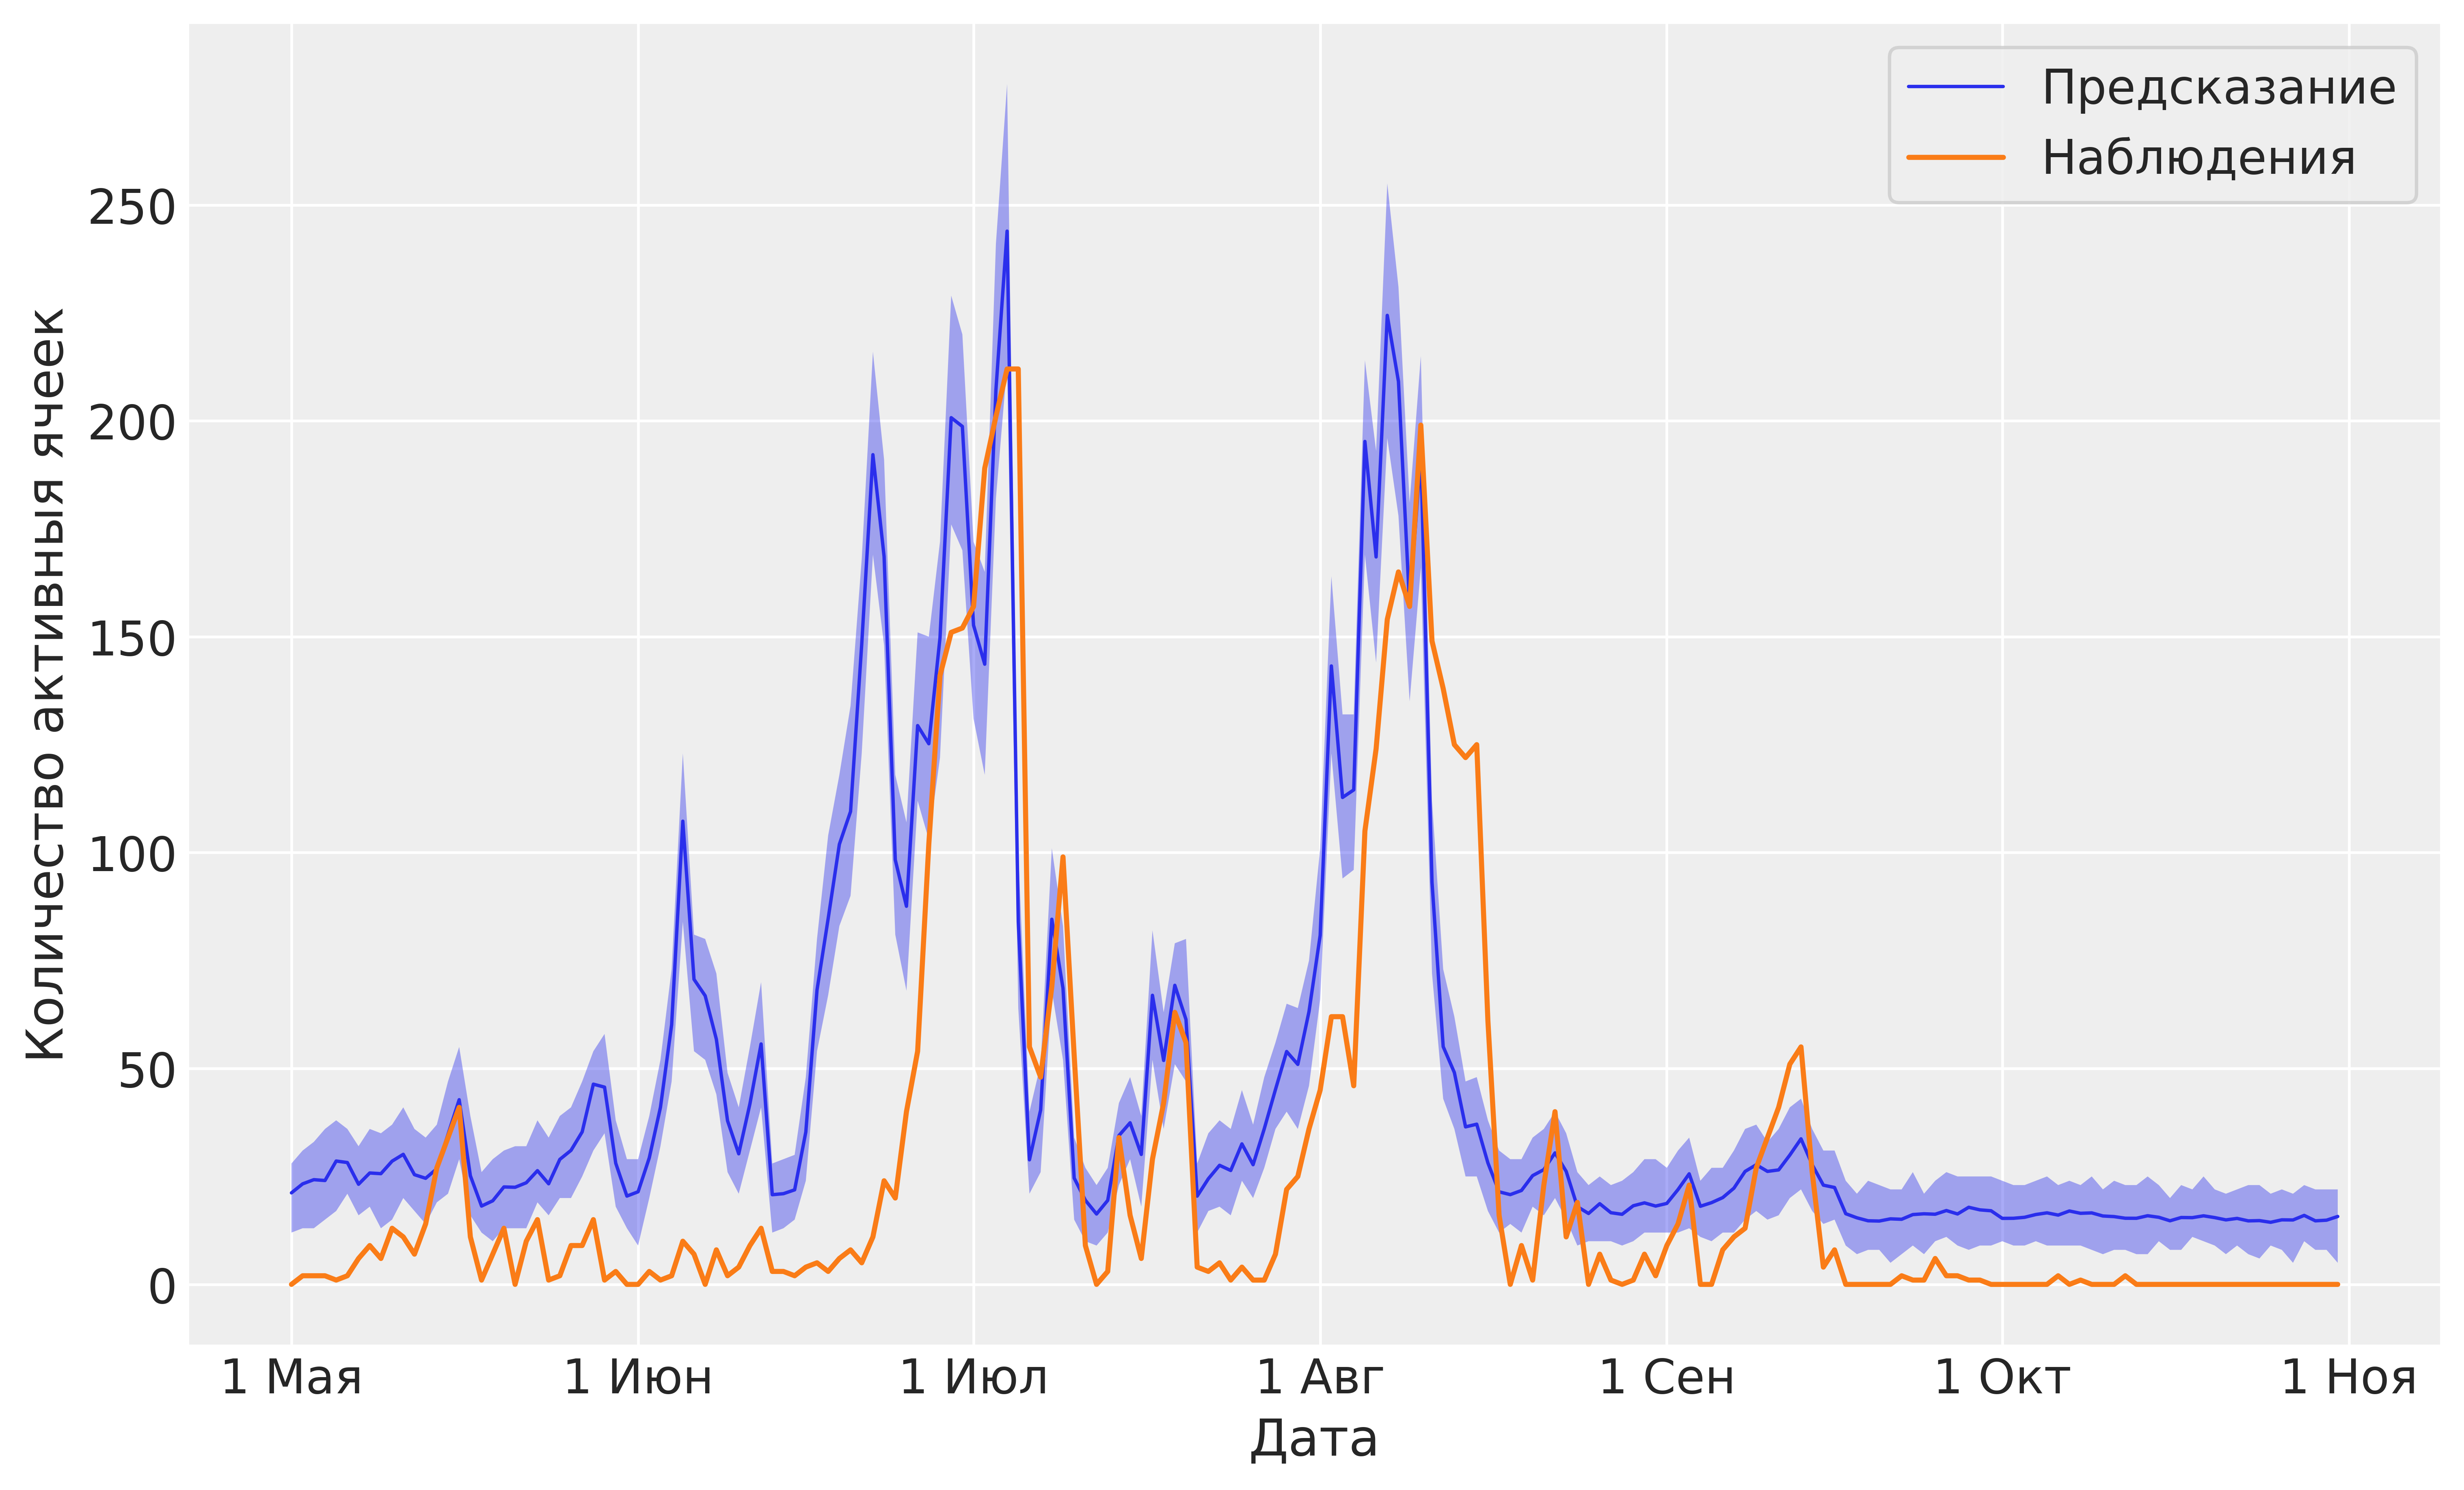
\includegraphics{images/glm_prediction.png}
}
\caption{
\label{cinema}
	Суточная динамика пожаров в регионе в 2021 году.}
\end {center}
\end {figure}

На графике предсказания модели в общих чартах повторяют динамику наблюдаемой величины. Однако видно, что большую часть периода низкой пожарной активности (первая половина июня, октябрь) предсказания модели стабильно превосходят наблюдения, которые также не укладываются в доверительный интервал.

Впрочем, если оценить пространственное распределение предсказаний, то даже в пиковый день предсказания модели значительно отличаются от реального географического распределения пожаров. На Рис. 2 слева изображены активные ячейки с активными лесными пожарами, а справа предсказанные моделью вероятности возникновения пожара. Как видно, предсказания лишь в очень общих чертах отражают пространственное распределение пожаров (увеличение по мере движения с севера на юг), а самые высокие значения вероятностей не совпадают с районами активных пожаров.

\begin{figure}[ht]
\begin{center}
\scalebox{0.5}{
	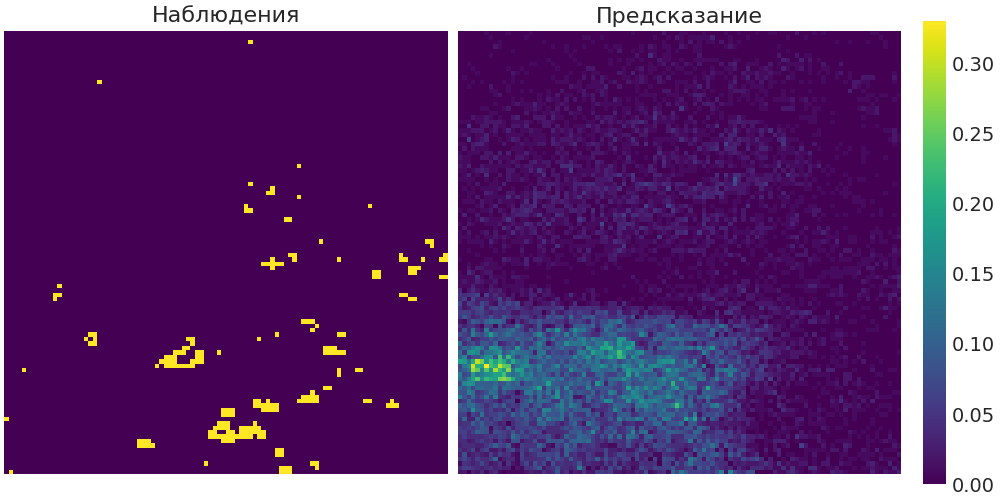
\includegraphics{images/glm_maps.png}
}
\caption{
\label{cinema}
	Пространственное распределение активных пожаров\\ и предсказаний GLM 4 июля.
}
\end {center}
\end {figure}

Хотя регрессия достаточно удачно воспроизвела динамику пожаров в регионе в целом, она не показала тех же успехов в точечных предсказаниях лесных пожаров в каждой ячейке. Вероятно, на качестве модели сказались простота моделируемой линейной взаимосвязи и недостаток пространственного компонента. Также вероятностная природа модели не дала ожидаемых преимуществ, как как доверительные интервалы едва ли свидетельствуют о высокой неопределенности предсказаний. Модель делает предсказания уверенно, но делает их ошибочно.

Результаты свидетельствуют о том, что даже для качества упрощенной бинарной классификации может потребоваться нелинейность предсказания и учет пространственной корелляции. FWI и лесной покров недостаточны для уверенного предсказания, так как не учитывают неприродные факторы, влияющие на лесные пожары.

\subsection{Нейросеть}

Однако нейронная сеть продемонстрировала еще меньшие успехи. В ходе обучений приблизительно после 15-й эпохи функция потерь практически перестала убывать (Рис. 3), и после 30-й эпохи обучение было остановлено. Итоговое значение метрики $F1$ для категоризации каждого пикселя составило всего $0.038$.

\begin{figure}[ht]
\begin{center}
\scalebox{0.4}{
	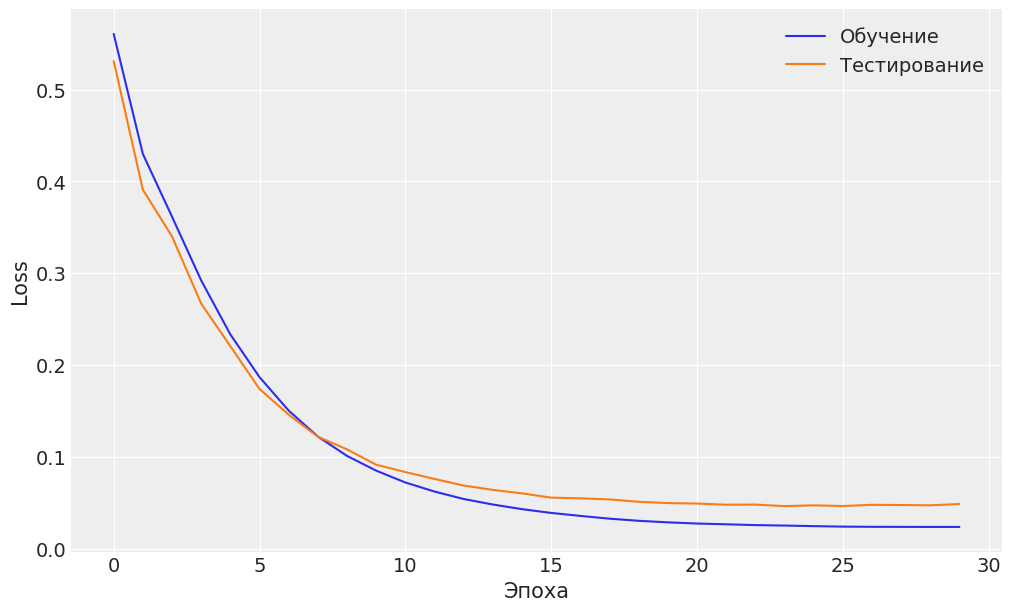
\includegraphics{images/unet_loss.png}
}
\caption{
\label{cinema}
	Кривые обучения.
}
\end {center}
\end {figure}

Основной проблемой предсказаний оказалось крайне низкие значений величин на выходе функции активации. На Рис. 4 изображена суточная предсказанная суточная динамика количества пожаров в зависимости от порога. Если значение пикселя оказывалось выше порогового, то данный пиксель определялся как активный. То есть, модель предсказывала в нем наличие лесного пожара. Как видно, уже при значении порога $0.2$ модель не предсказывает ни одного пожара за год вообще. При меньших значениях динамика наблюдаемой величины воспроизводится в общих чертах, но очень грубо.

\begin{figure}[ht]
\begin{center}
\scalebox{0.35}{
	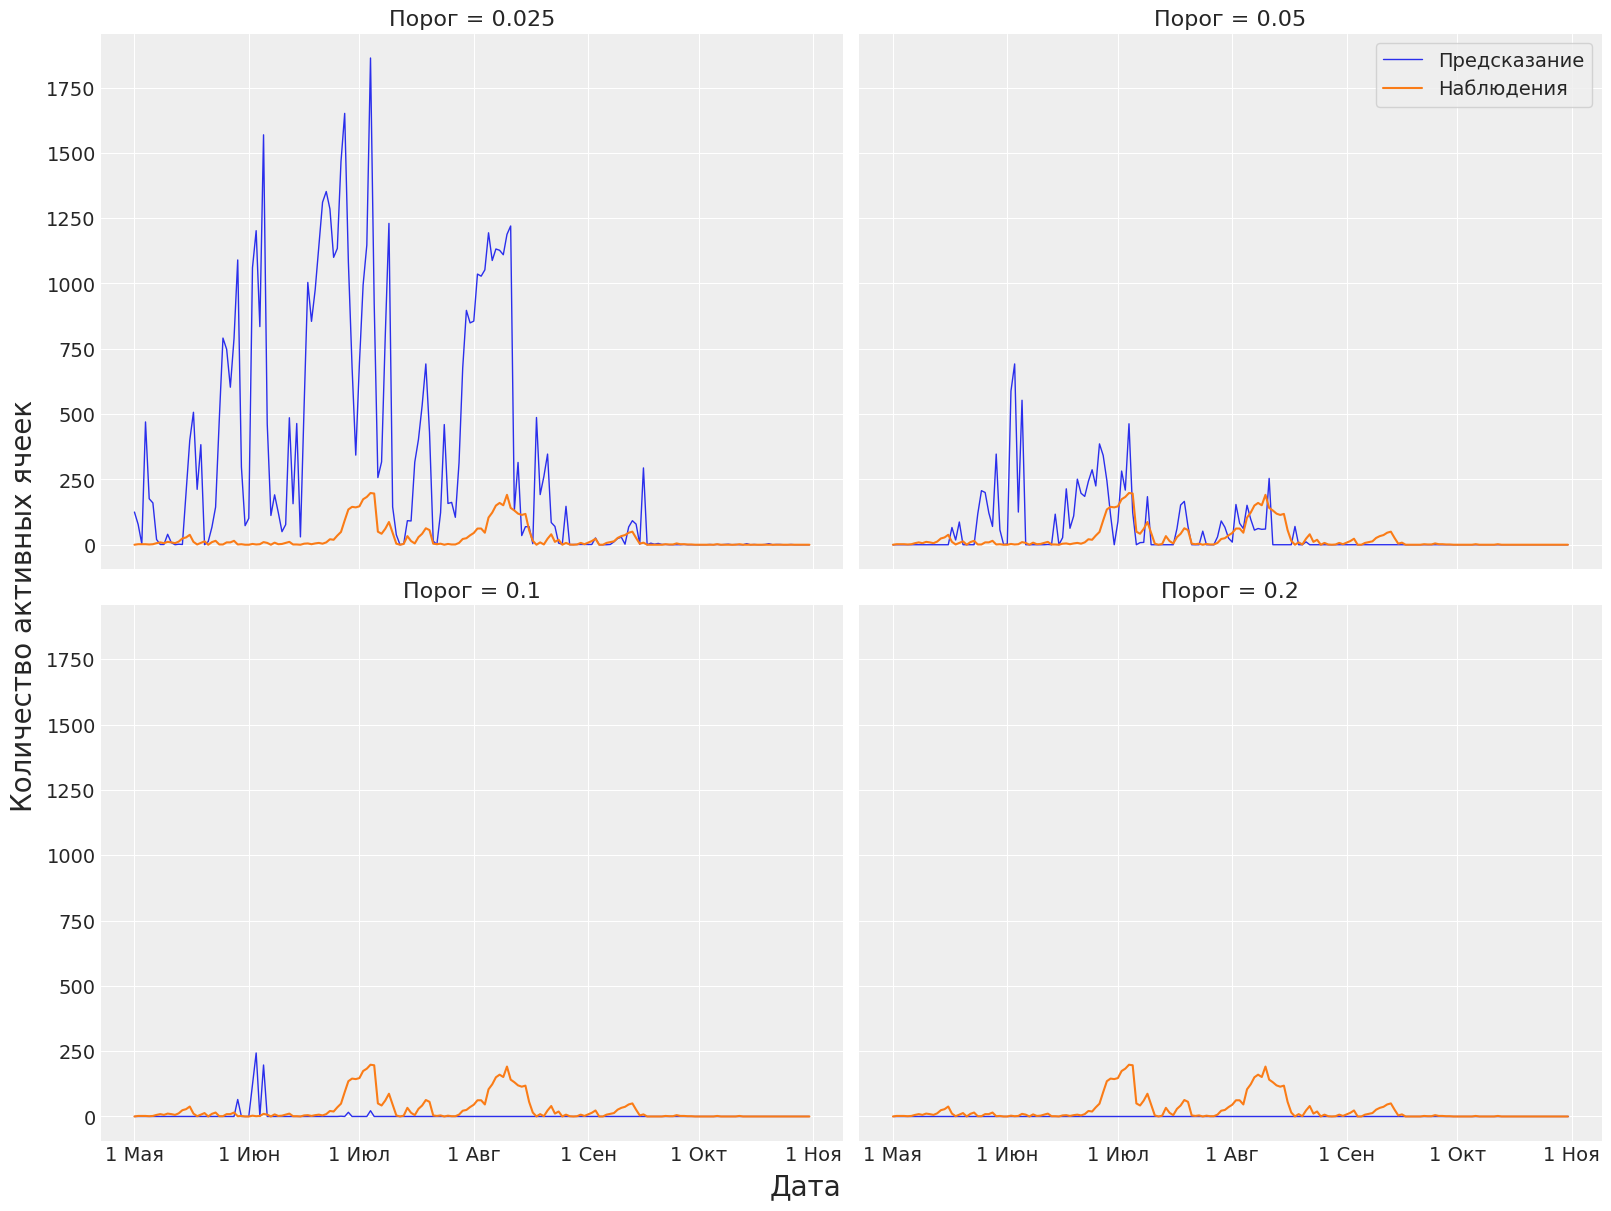
\includegraphics{images/unet_prediction.png}
}
\caption{
\label{cinema}
	Динамика активных пожаров и предсказаний U-Net\\ в зависимости от значения порога.
}
\end {center}
\end {figure}

Пространственная динамика также моделируется неудовлетворительно (Рис. 5). Вероятно, на качестве U-Net сказывается довольно разреженная структура целевой переменной, которая редко образует большие и непрерывные «пятна» активных областей, что отличает данную задачу от классической сегментации изображения, когда нейросеть имеет дело со сравнительно более крупными областями изображений. Также используемые изображения данных обладали меньшим разрешением, чем используемые в задачах компьютерного зрения.

Не оправдались ожидания от потенциала пространственного моделирования. Модель показывает себя даже хуже, чем логистическая регрессия, не содержащая пространственного фактора в принципе. В том числе, нейросеть неудачно показывает себя в воспроизведении пространственной структуры.

\begin{figure}[ht]
\begin{center}
\scalebox{0.5}{
	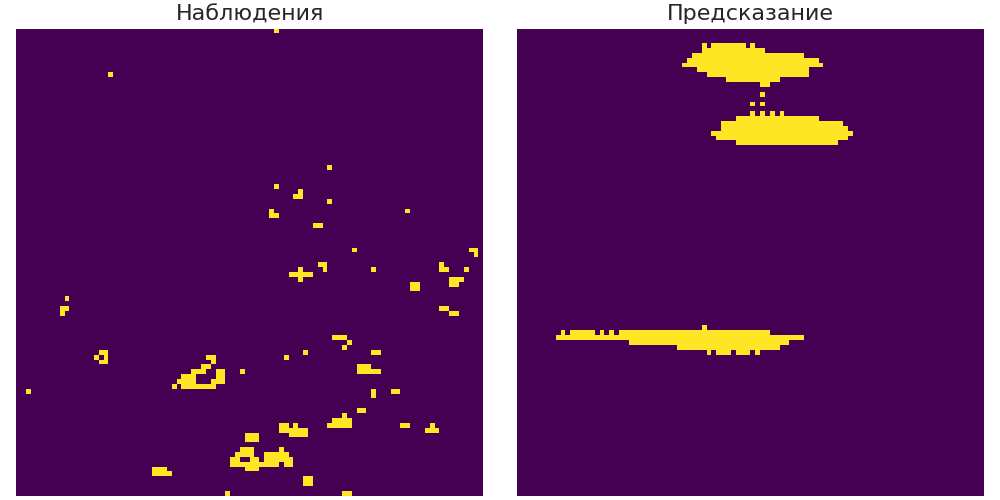
\includegraphics{images/unet_maps.png}
}
\caption{
\label{cinema}
	Пространственное распределение активных пожаров и предсказаний U-Net\\ при значении порога $0.05$ 4 июля.
}
\end {center}
\end {figure}

\pagebreak
\specialsection{Заключение}

В ходе работы был собран массив необходимых для моделирования пожарной активности данных для территории России. Из метеорологических показателей, данных дистанционного зондирования и радиоспектрометрии был составлен пространственно-временной датасет значений погодного пожарного индекса FWI, относительной площади лесного покрова и пожарной активности. Были построены две модели машинного обучения для предсказания пожарной активности на территории Дальнего Востока: байесовская логистическая регрессия и сверточная нейронная сеть U-Net.

Впрочем, обе построенные модели показали невыдающиеся результаты. Байесовская логистическая регрессия справилась лишь с одной из подзадач — предсказанием активности на уровне региона. Однако и этот результат нельзя называть успешным, так как качество предсказания все равно осталось низким. Насколько известно, ранее подобные модели не реализовывались в рамках прогнозирования пожарной активности на территории России. Притом  изученные в ходе работы методы основывались на иных источниках и представлениях данных, в значительной степени недоступных для России. В дальнейшем видится перспективным изучение сверточных нейросетей в решении указанной задачи, так как применение существующих архитектур не дает ожидаемых результатов.

\pagebreak
%TODO починить список литературы
\bibliographystyle{utf8gost705u}
\bibliography{biblio}


\end{document}
